\حصہء{سوالات}
\موٹا{خطوط}\\
سوال \حوالہ{سوال_مخروط_خط_قطبی_کارتیسی_الف}  تا سوال \حوالہ{سوال_مخروط_خط_قطبی_کارتیسی_ت} میں دیے خطوط کی قطبی اور کارتیسی مساوات تلاش کریں۔ 

\ابتدا{سوال}\شناخت{سوال_مخروط_خط_قطبی_کارتیسی_الف}
خط شکل \حوالہ{شکل_سوال_مخروط_خط_قطبی_کارتیسی_الف} میں ترسیم کیا گیا ہے۔
\انتہا{سوال}
%========================
\ابتدا{سوال}\شناخت{سوال_مخروط_خط_قطبی_کارتیسی_ب}
خط شکل \حوالہ{شکل_سوال_مخروط_خط_قطبی_کارتیسی_ب} میں ترسیم کیا گیا ہے۔
\انتہا{سوال}
%========================
\ابتدا{سوال}\شناخت{سوال_مخروط_خط_قطبی_کارتیسی_پ}
خط شکل \حوالہ{شکل_سوال_مخروط_خط_قطبی_کارتیسی_پ} میں ترسیم کیا گیا ہے۔
\انتہا{سوال}
%========================
\ابتدا{سوال}\شناخت{سوال_مخروط_خط_قطبی_کارتیسی_ت}
خط شکل \حوالہ{شکل_سوال_مخروط_خط_قطبی_کارتیسی_ت} میں ترسیم کیا گیا ہے۔
\انتہا{سوال}
%========================
\begin{figure}
\centering
\begin{minipage}{0.22\textwidth}
\centering
\begin{tikzpicture}[font=\scriptsize]
\pgfmathsetmacro{\a}{30}
\pgfmathsetmacro{\d}{2}
\draw[-latex](-0.15,0)--(3,0)node[right]{$x$};
\draw[-latex](0,-0.15)--(0,2)node[above]{$y$};
\draw(0,0)--++(\a:\d)coordinate(ka)node[pos=0.5,above]{$5$};
\draw[thick](\a:\d)++(\a-90:1.5)coordinate(kb)--++(\a+90:2.5);
\RightAngle{(0,0)}{(ka)}{(kb)}
\draw[-stealth]([shift={(0:0.5)}]0,0) arc (0:\a:0.5)node[right,yshift=-1ex]{$\tfrac{\pi}{6}$};
\end{tikzpicture}
\caption{ترسیم سوال \حوالہ{سوال_مخروط_خط_قطبی_کارتیسی_الف}}
\label{شکل_سوال_مخروط_خط_قطبی_کارتیسی_الف}
\end{minipage}\hfill
\begin{minipage}{0.22\textwidth}
\centering
\begin{tikzpicture}[font=\scriptsize]
\pgfmathsetmacro{\a}{135}
\pgfmathsetmacro{\d}{2}
\draw[-latex](-2.5,0)--(0.5,0)node[right]{$x$};
\draw[-latex](0,-0.15)--(0,2)node[above]{$y$};
\draw(0,0)--++(\a:\d)coordinate(ka)node[pos=0.5,above]{$2$};
\draw[thick](\a:\d)++(\a-90:1.5)coordinate(kb)--++(\a+90:2.5);
\RightAngle{(0,0)}{(ka)}{(kb)}
\draw[-stealth]([shift={(0:0.3)}]0,0) arc (0:\a:0.3)node[pos=0.25,above]{$\tfrac{3\pi}{4}$};
\end{tikzpicture}
\caption{ترسیم سوال \حوالہ{سوال_مخروط_خط_قطبی_کارتیسی_ب}}
\label{شکل_سوال_مخروط_خط_قطبی_کارتیسی_ب}
\end{minipage}\hfill
\begin{minipage}{0.22\textwidth}
\centering
\begin{tikzpicture}[font=\scriptsize]
\pgfmathsetmacro{\a}{240}
\pgfmathsetmacro{\d}{2}
\draw[-latex](-0.5,0)--(0.5,0)node[right]{$x$};
\draw[-latex](0,-0.15)--(0,0.5)node[above]{$y$};
\draw(0,0)--++(\a:\d)coordinate(ka)node[pos=0.5,above]{$3$};
\draw[thick](\a:\d)++(\a-90:1.5)coordinate(kb)--++(\a+90:2.5);
\RightAngle{(0,0)}{(ka)}{(kb)}
\draw[-stealth]([shift={(0:0.3)}]0,0) arc (0:\a:0.3)node[pos=0.75,above left]{$\tfrac{4\pi}{3}$};
\end{tikzpicture}
\caption{ترسیم سوال \حوالہ{سوال_مخروط_خط_قطبی_کارتیسی_پ}}
\label{شکل_سوال_مخروط_خط_قطبی_کارتیسی_پ}
\end{minipage}\hfill
\begin{minipage}{0.22\textwidth}
\centering
\begin{tikzpicture}[font=\scriptsize]
\pgfmathsetmacro{\a}{-45}
\pgfmathsetmacro{\d}{2}
\draw[-latex](-0.15,0)--(2,0)node[right]{$x$};
\draw[-latex](0,-0.15)--(0,0.25)node[above]{$y$};
\draw(0,0)--++(\a:\d)coordinate(ka)node[pos=0.5,below]{$4$};
\draw[thick](\a:\d)++(\a-90:1.5)coordinate(kb)--++(\a+90:2.5);
\RightAngle{(0,0)}{(ka)}{(kb)}
\draw[-stealth]([shift={(0:0.3)}]0,0) arc (0:\a:0.3)node[pos=0.8,right]{$-\tfrac{\pi}{4}$};
\end{tikzpicture}
\caption{ترسیم سوال \حوالہ{سوال_مخروط_خط_قطبی_کارتیسی_ت}}
\label{شکل_سوال_مخروط_خط_قطبی_کارتیسی_ت}
\end{minipage}
\end{figure}
